\begin{name}
	{ÔN TẬP KIỂM TRA CUỐI HỌC KÌ 1 - KNTT}
	{TOÁN 10}
	{LỚP TOÁN THẦY PHÁT}
	{\thoigian}
\end{name}

\caulc
\Opensolutionfile{ans}[ans/10-CK1-Chuyen-Hung-Vuong-Phan-1]


%MD-TH
\begin{ex}%[0D1H1-5]
	Cho mệnh đề $P\colon$\lq\lq $\forall x\in \mathbb{R},\, x^2-x+7< 0$\rq\rq. Mệnh đề phủ định của mệnh đề $P$ là
	\choice 
	{$\exists x\in \mathbb{R},\,x^2-x+7>0$}
	{$\forall x\in \mathbb{R},\,x^2-x+7>0$} 
	{$\forall x\notin \mathbb{R},\,x^2-x+7\ge 0$}
	{\True $\exists x\in \mathbb{R},\,x^2-x+7\ge 0$} 
	\loigiai{
		Phủ định của mệnh đề $P$ là $\overline{P}\colon$\lq\lq $\exists x\in \mathbb{R},\, x^2-x+7\ge 0$\rq\rq.
	}
\end{ex}

\begin{ex}%[0D1H2-1]
	Cho tập hợp $A= \{x \in \mathbb{Z}\, \mid \, x^2<17 \} $. Khẳng định nào sau đây là \textbf{đúng}?
	\choice
	{\True $A= \{ x \in \mathbb{Z} \mid -4 \le x \le 4 \} $}
	{$A= \{ x \in \mathbb{Z} \mid -4 < x < 4 \} $}
	{$A=(-4;4) $}
	{$A= [-4;4] $}
		\loigiai{Ta có $x^2<17\Leftrightarrow \left|x\right|<\sqrt{17}\Leftrightarrow -\sqrt{17}<x<\sqrt{17}$.\\
				Vì $x\in \mathbb{Z}$ nên $A=\{ -4;-3;-2;-1;0;1;2;3;4 \} $.
			}
\end{ex}

%BPT

\begin{ex}%[0D2N1-2]
	Cặp số nào sau đây là một nghiệm của bất phương trình $x + 2y \le 4$?
	\choice
	{\True $(2; 1)$}
	{$(1; 2)$}
	{$(1; 3)$}
	{$(-1; 3)$}
	\loigiai{
		Chỉ có $(2; 1)$ là nghiệm của bất phương trình $x + 2y \le 4$.\\ Vì $2 + 2\cdot 1 \le 4$.
	}
\end{ex}

\begin{ex}%[0D2N2-1]
	Trong các hệ sau,  hệ nào \textbf{không} là hệ bất phương trình bậc nhất hai ẩn?
	\choice
	{$ \heva{& x+y>0  \\&  x>1}$}
	{\True $\True \heva{& x+y<-2  \\&  x^2>5}$}
	{$ \heva{& 2 x+3 y>10  \\&  x-4 y< 1}$}
	{$ \heva{& y>0  \\&  x-4 \leqslant 1}$}
	\loigiai{Hệ $ \heva{& x+y<-2  \\&  x^2>5} $ không phải hệ bất phương trình bậc nhất hai ẩn vì $x^2>5$ là bất phương trình bậc hai.}
\end{ex}

%HTL
\begin{ex}%[0H4H2-1]
	Cho tam giác $A B C$ có các góc thoả mãn $\dfrac{\sin A}{1}=\dfrac{\sin B}{2}=\dfrac{\sin C}{\sqrt{3}}$. Tính số đo $\widehat{A}$ của tam giác.
	\choice
	{$\widehat{A}=60^{\circ}$}
	{\True $\widehat{A}=30^{\circ}$}
	{$\widehat{A}=45^{\circ}$}
	{$\widehat{A}=90^{\circ}$}
	\loigiai{
		Áp dụng định lí Sin ta được  $a: b: c=1: 2: \sqrt{3} \Rightarrow \heva{&b=2a\\&c=\sqrt{3}a.}$\\
		Áp dụng định lí Cô-sin, ta có $\cos A= \dfrac{b^2+c^2-a^2}{2bc}=\dfrac{\sqrt{3}}{2} \Rightarrow \widehat{A}=30^\circ.$\\
		Vậy $\widehat{A}=30^{\circ}$.
	}
\end{ex}

\begin{ex}%[0H4H2-1]
	Cho tam giác $ABC$ có $AB = 9$, $AC=10$, $BC=17$. Giá trị $\cos A$ là
	\choice
	{\True $-\dfrac{3}{5}$}
	{$\dfrac{3}{5}$}
	{$-\dfrac{5}{3}$}
	{$\dfrac{5}{3}$}
	\loigiai{
		Định lí cô-sin trong tam giác $ABC$.
		\begin{align*}
			BC^2 &= AC^2 + AB^2 - 2\cdot AC\cdot AB \cdot \cos A\\ \Rightarrow \cos A &= \dfrac{AC^2 + AB^2 - BC^2 }{2\cdot AC \cdot AB} \\
			&= \dfrac{10^2 + 9^2 - 17^2}{2\cdot 10 \cdot 9}\\
			&= -\dfrac{3}{5}. 
		\end{align*}
	}
\end{ex}

%Vecto
\begin{ex}%[0H5N1-3]
	Khẳng định nào sau đây \textbf{đúng}?
	\choice
	{Hai vectơ đối nhau nếu chúng cùng độ dài}
	{Hai vectơ đối nhau nếu chúng ngược hướng}
	{Hai vectơ đối nhau nếu chúng cùng phương và cùng độ dài}
	{\True Hai vectơ đối nhau nếu chúng ngược hướng và cùng độ dài}
	\loigiai{
	Hai vectơ đối nhau nếu chúng ngược hướng và cùng độ dài.
	}
\end{ex}

\begin{ex}
	\immini{Cho hình chữ nhật $ABCD$, khẳng định nào sau đây đúng?
		\choice
		{$\overrightarrow{AB}=\overrightarrow{CD}$}
		{$\overrightarrow{AC}=\overrightarrow{BD}$}
		{$\overrightarrow{CA}=\overrightarrow{BD}$}
		{\True $\overrightarrow{AD}=\overrightarrow{BC}$}
	}
	{
		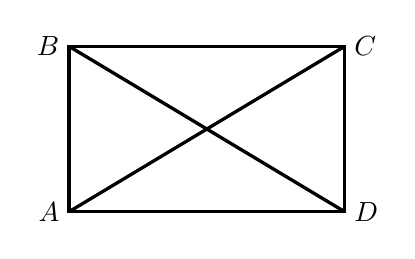
\begin{tikzpicture}[scale=0.7]
			\draw[very thick] (0,0) rectangle (5,3);
			\draw (0,0) node[left]{$A$} (0,3) node[left]{$B$} (5,3) node[right]{$C$} (5,0) node[right]{$D$};
			\draw[very thick] (0,0)--(5,3) (0,3)--(5,0);
		\end{tikzpicture}
	}
\end{ex}

\begin{ex}%[0H2H2-1]
	Cho hình vuông $ABCD$ cạnh $a$. Tích vô hướng của hai vectơ $\overrightarrow{AB}$ và $\overrightarrow{AC}$ là
	\choice
	{$a\sqrt{2}$}
	{$2a$}
	{\True $a^2$}
	{$2a^2$}
	\loigiai{
		Ta có $\overrightarrow{AB}\cdot\overrightarrow{AC}=|\overrightarrow{AB}|\cdot|\overrightarrow{AC}|\cdot\cos(\overrightarrow{AB},\overrightarrow{AC})=a\cdot a\sqrt{2}\cos 45^\circ=a^2$.
	}
\end{ex}

\begin{ex}%[0H9H1-3]
	Trong mặt phẳng với hệ tọa độ $Oxy$, cho ba điểm $A(1;1)$, $B(3;2)$, $C(6;5)$. Tìm tọa độ điểm $D$ để $ABCD$ là hình bình hành.
	\choice
	{\True $(4;4)$}
	{$(3;4)$}
	{$(4;3)$}
	{$(8;6)$}
	\loigiai{
		Ta có $\overrightarrow{AB}=(2;1)$, $\overrightarrow{BC}=(3;3)$. Ta thấy $\dfrac{2}{3}\ne\dfrac{1}{3}$ nên hai vectơ $\overrightarrow{AB}$ và $\overrightarrow{BC}$ không cùng phương. Do đó, ba điểm $A$, $B$, $C$ không thẳng hàng.\\
		Gọi $D(x;y)$. Khi đó, $\overrightarrow{AD}=(x-1;y-1)$.\\
		$ABCD$ là hình bình hành khi và chỉ khi $\overrightarrow{AD}=\overrightarrow{BC}$ $\Leftrightarrow$ $\heva{&x-1=3\\ &y-1=3}$ $\Leftrightarrow$ $\heva{&x=4\\ &y=4.}$\\
		Vậy $D(4;4)$.
	}
\end{ex}

%Thong ke
\begin{ex}%[0D6N3-5] 
	Khẳng định nào sau đây \textbf{đúng}?
	\choice
	{\True Mốt của mẫu số liệu là giá trị xuất hiện với tần số lớn nhất}
	{Mốt của mẫu số liệu là giá trị xuất hiện với tần số nhỏ nhất}
	{Mốt của mẫu số liệu là giá trị lớn nhất trong mẫu số liệu}
	{Mốt của mẫu số liệu là giá trị nhỏ nhất trong mẫu số liệu}
	\loigiai{
	Mốt của mẫu số liệu là giá trị xuất hiện với tần số lớn nhất.
	}
\end{ex}

\begin{ex}%[0D6N3-3] 
	Khẳng định nào sau đây đúng?
	\choice
	{Số trung bình không bị ảnh hưởng bởi giá trị bất thường}
	{Số trung bình và số trung vị đều là các số đặc trưng đo độ phân tán của một mẫu số liệu}
	{\True Số trung vị không bị ảnh hưởng bởi giá trị bất thường}
	{Số trung bình là giá trị chia đôi mẫu số liệu}
	\loigiai{
	Số trung bình bị ảnh hưởng bởi giá trị bất thường, trong khi số trung vị thì không bị ảnh hưởng.
	}
\end{ex}

\Closesolutionfile{ans}
% \indapan{7}{ans/10-CK1-Chuyen-Hung-Vuong-Phan-1}

\cauds
\Opensolutionfile{ans}[ans/10-CK1-Toan-Tu-Tam-Phan-2]
%%%%==============Cau_EX1==============%%%
% \begin{ex}%[0H4H1-3]
% 	Cho góc lượng giác $\alpha$ thỏa mãn $\cos \alpha=\dfrac{1}{3}$ và $0^\circ < \alpha < 90^\circ$. Các mệnh đề sau đúng hay sai?	
% 	\choiceTF
% 	{\True $\tan \alpha > 0$}
% 	{$\sin \left(90^\circ+\alpha \right)=\dfrac{2}{3}$}
% 	{\True Giá trị $\tan \alpha=2\sqrt{2}$}
% 	{\True $\dfrac{1+\sin ^2\alpha}{1-\sin ^2\alpha}=1+2\tan ^2\alpha$}
% 	\loigiai{
% 		\begin{itemchoice}
% 			\itemch \textbf{Đúng.}\\
% 			Vì $0^\circ < \alpha < 90^\circ$ nên $\tan \alpha > 0$.
% 			\itemch \textbf{Sai.}\\
% 			Ta có $\sin \left(90^\circ+\alpha \right)=\sin \left(180^\circ-90^\circ-\alpha \right)=\sin \left(90^\circ-\alpha \right)=\cos \alpha=\dfrac{1}{3}$.
% 			\itemch \textbf{Đúng.}\\
% 			Ta có $\tan ^2\alpha+1=\dfrac{1}{\cos ^2\alpha} \Leftrightarrow \tan ^2\alpha+1=9\Leftrightarrow \tan ^2\alpha=8\Leftrightarrow \tan \alpha=2\sqrt{2}$ (vì $\tan \alpha > 0$).
% 			\itemch \textbf{Đúng.}\\
% 			Ta có $\dfrac{1+\sin ^2\alpha}{1-\sin ^2\alpha}=\dfrac{1+\sin ^2\alpha}{\cos ^2\alpha}=\dfrac{1}{\cos ^2\alpha}+\dfrac{\sin ^2\alpha}{\cos ^2\alpha}=\tan ^2\alpha+1+\tan ^2\alpha=2\tan ^2\alpha+1$
% 			\end{itemchoice}
% 			}
% 		\end{ex}
% \begin{ex}%[0D3V2-1]
% 	 Cho hàm số $y=ax^2+bx+2$ với $a\ne 0$, có đồ thị là $\left(P\right)$. Các mệnh đề sau đúng hay sai?
% \choiceTF
% 	{Biết $\left(P\right)$ đi qua điểm $E\left(-1;5\right)$. Khi đó $a-b=4$}
% 	{Biết $\left(P\right)$ có trục đối xứng là đường thẳng $x=1$, khi đó $2a-b=0$}
% 	{\True Biết $\left(P\right)$ đi qua hai điểm $M\left(1;0\right)$ và $N\left(-1;0\right)$, khi đó $a+2024b=-2$}
% 	{\True Biết $\left(P\right)$ có đỉnh là điểm $S\left(-1;-\dfrac{3}{2} \right)$. Khi đó $\left(2a+b\right)\; \vdots \; 14$}
% \loigiai{
% \begin{itemchoice}
% 	\itemch \textbf{Sai.}\\
% 	$\left(P\right)$ đi qua điểm $E\left(-1;5\right)$ nên $a-b+2=5\Leftrightarrow a-b=3$.
% 	\itemch \textbf{Sai.}\\
% 	$\left(P\right)$ có trục đối xứng là đường thẳng $x=1$, khi đó $-\dfrac{b}{2a}=1\Leftrightarrow 2a+b=0$.
% 	\itemch \textbf{Đúng.}\\
% 	$\left(P\right)$ đi qua hai điểm $M\left(1;0\right)$ và $N\left(-1;0\right)$ nên ta được
% 	\[\heva{&a+b+2=0 \\ &a-b+2=0}  \Leftrightarrow \heva{ &a=-2 \\ & b=0} \Rightarrow a+2024b=-2.	\]
% 	\itemch \textbf{Đúng.}\\
% 	Vì $\left(P\right)$ có đỉnh là điểm $S\left(-1;-\dfrac{3}{2} \right)$ nên hoành độ đỉnh \[x=-1=-\dfrac{b}{2a} \Rightarrow 2a-b=0\; \qquad\qquad(1)\]
% 	Lại có $\left(P\right)$ đi qua $S\left(-1;-\dfrac{3}{2} \right)$ nên $a-b+2=-\dfrac{3}{2} \Leftrightarrow a-b=-\dfrac{7}{2} \; (2)$.\\
% 	Từ $(1)$, $(2)$ ta được $a=\dfrac{7}{2}$, $b=7\Rightarrow 2a+b=14$ nên chia hết cho $14$.
% \end{itemchoice}
% }
% \end{ex}
\begin{ex}%[0D6H4-2]
	 Điểm trung bình các môn trong kỳ thi tốt nghiệp trung học phổ thông năm 2024 được thống kê trong bảng sau:
\begin{center}
	\begin{tabular}{|c|c|c|c|c|c|c|c|c|c|}
		\hline
	Môn & Toán & Văn & Vật lý& Hóa học & Sinh học & Lịch sử & Địa lý & GDCD & Ngoại ngữ \\ 
	\hline
	Điểm & $6{,}45$& $7{,}23$& $6{,}67$& $6{,}68$& $6{,}28$ &$6{,}57$ & $7{,}19$ & $8{,}16$& $5{,}51$\\
	\hline
	\end{tabular}
\end{center}
Các khẳng định sau đúng hay sai?
\choiceTF
{\True Điểm trung bình của 9 môn thi tốt nghiệp năm 2024 (làm tròn đến hàng phần trăm) là $6{,}75$}
{Điểm trung bình của các môn thuộc tổ hợp khoa học tự nhiên (Vật lý, Hóa học, Sinh học) cao hơn điểm trung bình của các môn thuộc tổ hợp khoa học xã hội (Lịch sử, Địa lý, GDCD)}
{Trung vị của mẫu số liệu trên là $6{,}68$}
{\True Khoảng biến thiên của mẫu số liệu trên là $2{,}65$}
\loigiai{
\begin{itemchoice}
	\itemch \textbf{Đúng.}\\
	Điểm trung bình của $9$ môn thi tốt nghiệp năm $2\,024$ là \[\overline{x}=\dfrac{6{,}45+7{,}23+6{,}67+6{,}68+6{,}28+6{,}57+7{,}19+8{,}16+5{,}51}{9}=\dfrac{3037}{450} \approx 6{,}75.\]
	\itemch \textbf{Sai.}\\
	Điểm trung bình của các môn thuộc tổ hợp khoa học tự nhiên (Vật lý, Hóa học, Sinh học) là 
	\[\overline{x}_1=\dfrac{6{,}67+6{,}68+6{,}28}{3}=\dfrac{1963}{300} \approx 6{,}54.\]
	Điểm trung bình của các môn thuộc tổ hợp khoa học xã hội (Lịch sử, Địa lý, GDCD) là 	\[\overline{x}_2=\dfrac{6{,}57+7{,}19+8{,}16}{3}=\dfrac{548}{75} \approx 7{,}31.\]
	Suy ra điểm trung bình của các môn thuộc tổ hợp khoa học tự nhiên (Vật lý, Hóa học, Sinh học) thấp hơn điểm trung bình của các môn thuộc tổ hợp khoa học xã hội (Lịch sử, Địa lý, GDCD).
	\itemch \textbf{Sai.}\\
	Sắp xếp mẫu số liệu trên theo thứ tự không giảm ta được dãy sau
	\[5{,}51;\, 6{,}28;\, 6{,}45;\, 6{,}57;\, 6{,}67; \,6{,}68;\, 7{,}19;\, 7{,}23;\, 8{,}16\]
	Vì cỡ mẫu là $9$ nên giá trị trung vị là $x_5=6{,}67$.
	\itemch \textbf{Đúng.}\\
	Giá trị bé nhất của mẫu số liệu trên là $5{,}51$.\\
	Giá trị lớn nhất của mẫu số liệu trên là $8{,}16$.\\
	Do đó khoảng biến thiên của mẫu số liệu trên là $8{,}16-5{,}51=2{,}65$.
	\end{itemchoice}
}
\end{ex}
\begin{ex}%[0H5V4-6]
	 Cho hình vuông $ABCD$ với độ dài cạnh bằng $a$. Các khẳng định sau đúng hay sai?
\choiceTF
{\True $\overrightarrow{BC}+\overrightarrow{BA}=\overrightarrow{BD}$}
{Độ dài của vectơ $\overrightarrow{AB}+\overrightarrow{CB}$ bằng $2a$}
{$\overrightarrow{BA}\cdot \overrightarrow{DB}=a^2$}
{Với điểm $M$ bất kỳ, gọi $T=\left|\overrightarrow{MA}+\overrightarrow{MB}+\overrightarrow{MC}+\overrightarrow{MD}\right|$. Giá trị nhỏ nhất của $T$ là $2024a$}
\loigiai{
\begin{itemchoice}
	\itemch \textbf{Đúng.}\\
	Theo quy tắc hình bình hành ta có $\overrightarrow{BC}+\overrightarrow{BA}=\overrightarrow{BD}$.
	\itemch \textbf{Sai.}\\
	Do $\overrightarrow{AB}=\overrightarrow{DC}$ nên $\overrightarrow{AB}+\overrightarrow{CB}=\overrightarrow{DC}+\overrightarrow{CB}=\overrightarrow{DB}$.\\
	Vậy $\left|\overrightarrow{AB}+\overrightarrow{CB}\right|=\left|\overrightarrow{DB}\right|=DB=a\sqrt{2}$.
	\itemch \textbf{Sai.}\\
	Ta có 
	\begin{align*}
		\overrightarrow{BA}\cdot \overrightarrow{DB} &=-\overrightarrow{BA}\cdot \overrightarrow{BD}\\
		&=-\left|\overrightarrow{BA}\right|\cdot\left|\overrightarrow{BD}\right|\cos\left(\overrightarrow{BA}; \overrightarrow{BD}\right)\\
		&=-a\cdot a\sqrt{2} \cos45^\circ=-a\cdot a\sqrt{2}\cdot \dfrac{\sqrt{2}}{2}=-a^2.		
	\end{align*}
	\itemch \textbf{Sai.}\\
	Gọi $O$ là tâm hình vuông $ABCD$, ta có
	\begin{align*}
		T &=\left|\overrightarrow{MA}+\overrightarrow{MB}+ \overrightarrow{MC}+\overrightarrow{MD}\right|\\
		&=\left|\overrightarrow{MO}+\overrightarrow{OA}+\overrightarrow{MO}+\overrightarrow{OB}+\overrightarrow{MO}+\overrightarrow{OC}+\overrightarrow{MO}+\overrightarrow{OD}\right|\\
		&=\left|4\overrightarrow{MO}+\overrightarrow{OA}+\overrightarrow{OB}+\overrightarrow{OC}+\overrightarrow{OD}\right|=\left|4\overrightarrow{MO}\right|=4MO\ge 0\\
		T&=0\Leftrightarrow M\equiv O .
	\end{align*}
	Vậy $T$ nhỏ nhất là $0$, đạt được khi $M\equiv O$.
	\end{itemchoice}
	}
\end{ex}
\Closesolutionfile{ans}
% \indapan{3}{ans/10-CK1-Toan-Tu-Tam-Phan-2}
\caukq
\Opensolutionfile{ans}[ans/10-CK1-Toan-Tu-Tam-Phan-3]
\begin{ex}%[2D1V1-5] 
	Ở một giải đua ô tô địa hình, một vận động cần hoàn thành chặng đường từ $A$ đến $B$ gồm $3$ đoạn: đường bằng, leo dốc và xuống dốc như hình vẽ bên dưới. Trên đoạn đường bằng $AC$ dài $10$km, xe chạy với vận tốc $100$km/h. Xe leo dốc $CD$ với vận tốc là $10$ km/h và xe xuống dốc $DB$ với vận tốc là $50$ km/h. Biết rằng: $BC=20$ km, $\widehat{DCB}=45^\circ$ và $\widehat{DBC}=30^\circ$. Hỏi vận động viên mất bao nhiêu giờ để hoàn thành chặng đường từ $A$ đến $B$? (các kết quả làm tròn đến hàng phần trăm).
	\begin{center}
		\begin{tikzpicture}[scale=1, line cap=round, line join=round, font=\footnotesize,>=stealth]
			\def\a{2}
			\path (0,0) coordinate (A) (0:\a) coordinate (C)++(45:.1)coordinate (c)
			(0:3*\a)coordinate (B)++(150:.1) coordinate (b)
			(intersection of C--c and B--b) coordinate (D);
			\draw (A)--(C)--(D)--(B);
			\foreach \a/\b in {A/-90,C/-90,D/40,B/-30}{
				\fill[black] (\a)circle(.7pt) ($(\a)+(\b:2mm)$)node[scale=.8]{$\a$};
			}
		\end{tikzpicture}
	\end{center}
	
	\shortans[oly]{1,43}
	\loigiai{
		Thời gian xe chạy trên đoạn đường bằng là $t_1=\dfrac{10}{100}=\dfrac{1}{10}$ (h).\\
		\begin{center}
			\begin{tikzpicture}[scale=1, line cap=round, line join=round, font=\footnotesize,>=stealth]
				\def\a{2}
				\path (0,0) coordinate (A) (0:\a) coordinate (C)++(45:.1)coordinate (c)
				(0:3*\a)coordinate (B)++(150:.1) coordinate (b)
				(intersection of C--c and B--b) coordinate (D);
				\draw pic[draw, angle radius=2mm, angle eccentricity=2.5, "\tiny $45^\circ$"]{angle= B--C--D};
				\draw pic[draw,double, angle radius=3mm, angle eccentricity=2, "\tiny $30^\circ$"]{angle= D--B--C};
				\draw (A)--(C)--(D)--(B)--(C);
				\foreach \a/\b in {A/-90,C/-90,D/40,B/-30}{
					\fill[black] (\a)circle(.7pt) ($(\a)+(\b:2mm)$)node[scale=.8]{$\a$};
				}
			\end{tikzpicture}
		\end{center}
		Ta có $\widehat{BDC}=180^\circ -\left(\widehat{DCB}+\widehat{DBC}\right)=105^\circ$.\\
		Áp dụng định lý sin trong $\triangle BCD$, ta có
		$\dfrac{BC}{\sin \widehat{BDC}}=\dfrac{CD}{\sin \widehat{DBC}}=\dfrac{BD}{\sin \widehat{DCB}}$.\\
		Suy ra $CD=\dfrac{20\cdot \sin 30^\circ}{\sin 105^\circ}=10\sqrt{6}-10\sqrt{2}$ (km) và $BD=\dfrac{20\cdot \sin 45^\circ}{\sin 105^\circ}=20\sqrt{3}-20$ (km).\\
		Thời gian xe chạy trên đoạn đường leo dốc là $t_2=\dfrac{10\sqrt{6}-10\sqrt{2}}{10}=\sqrt{6}-\sqrt{2}$ (h).\\
		Thời gian xe chạy trên đoạn đường xuống dốc là $t_3=\dfrac{20\sqrt{3}-20}{50}=\dfrac{2\sqrt{3}-2}{5}$ (h).\\
		Tổng thời gian vận động viên hoàn thành chặng đường từ $A$ đến $B$ là
		\[t_1+t_2+t_3=\dfrac{1}{10}+\sqrt{6}-\sqrt{2}+\dfrac{2\sqrt{3}-2}{5}\approx 1{,}43 \mathrm{~(h)}.\]
		Vậy vận động viên mất $1{,}43$ giờ để hoàn thành chặng đường từ $A$ đến $B$.
	}
\end{ex}
% \begin{ex}%[2D1V1-5]
% 	Hàm số $y=\sqrt{1-x}+\sqrt{x+2}$ có tập xác định là $\mathscr{D}=\left[a;b\right]$. Tính $a+2b$.
	
% 	\shortans[oly]{0}
% 	\loigiai{
% 		Hàm số $y=\sqrt{1-x}+\sqrt{x+2}$ xác định khi 
% 		$\heva{&1-x\ge 0 \\&x+2\ge 0}\Leftrightarrow \heva{&x\le 1 \\&x\ge -2}
% 		\Leftrightarrow -2\le x\le 1$.\\
% 		Hay tập xác định của hàm số đã cho là $\mathscr{D}=[-2; 1]$.\\
% 		Do đó $a=-2$, $b=1$.\\ Vậy $a+2b=0$.
% 	}
% \end{ex}
% \begin{ex}%[2D1V3-6]
% 	Một doanh nghiệp tư nhân chuyên kinh doanh tủ lạnh các loại. Hiện nay doanh nghiệp đang tập trung chiến lược vào kinh doanh tủ lạnh Hitachi với chi phí mua vào một chiếc là $27$ triệu đồng và bán ra với giá là $31$ triệu đồng. Với giá bán này thì số lượng tủ lạnh mà khách hàng sẽ mua trong một năm là $600$ chiếc. Nhằm mục tiêu đẩy mạnh hơn nữa lượng tiêu thụ dòng tủ lạnh đang ăn khách này, doanh nghiệp dự định giảm giá bán và ước tính rằng nếu giảm $1$ triệu đồng mỗi chiếc tủ lạnh thì số lượng tủ lạnh bán ra trong một năm là sẽ tăng thêm $200$ chiếc. Vậy doanh nghiệp phải định giá bán mới là bao nhiêu để sau khi đã thực hiện giảm giá, lợi nhuận thu được sẽ là cao nhất?
	
% 	\shortans[oly]{30,5}
% 	\loigiai{
% 		Gọi $x$ triệu đồng là số tiền mà doanh nghiệp $A$ dự định giảm giá; $(0\le x\le 4)$.
% 		Khi đó
% 		\begin{itemize}
% 			\item Lợi nhuận thu được khi bán một chiếc tủ lạnh là $31-x-27=4-x$.
% 			\item Số xe mà doanh nghiệp sẽ bán được trong một năm là $600+200x$.
% 			\item Lợi nhuận mà doanh nghiệp thu được trong một năm là
% 			\[f(x)=(4-x)(600+200x)=-200x^2+200x+2400.\]
% 		\end{itemize}
% 		Xét hàm số $f(x)=-200x^2+200x+2400$ trên đoạn $[0;4]$ có bảng biến thiên
% 		\begin{center}
% 			\begin{tikzpicture}[scale=1, font=\footnotesize, line join=round, line cap=round, >=stealth]
% 				\tkzTabInit[nocadre=false,lgt=1,espcl=2,deltacl=0.5]
% 				{$x$/.7 ,$y'$/.7,$y$/2}
% 				{$0$ , $\tfrac{1}{2}$ , $4$}
% 				\tkzTabLine{ , + , $0$ , - , }
% 				\tkzTabVar{-/$2400$ , +/$2450$ , -/$0$}
% 			\end{tikzpicture}
% 		\end{center}
% 		Vậy giá trị lớn nhất của hàm số $f(x)$ bằng $2\, 450$ (triệu) khi $x=\dfrac{1}{2}$.\\
% 		Vậy giá mới của chiếc xe là $30{,}5$ triệu đồng thì lợi nhuận thu được là cao nhất.
% 	}
% \end{ex}
\begin{ex}% [2H2V2-6] 
	Cho ba lực $\overrightarrow{F}_1=\overrightarrow{MA}$, $\overrightarrow{F}_2=\overrightarrow{MB}$, $\overrightarrow{F}_3=\overrightarrow{MC}$ cùng tác động vào một ô tô tại điểm $M$ và ô tô đứng yên. Cho biết cường độ hai lực $\overrightarrow{F}_1$, $\overrightarrow{F}_2$ đều bằng $25$N và góc $\widehat{AMB}=60^\circ$. Khi đó tính cường độ $\overrightarrow{F}_3$ (làm tròn đến hàng phần chục).
		\begin{center}
		\begin{tikzpicture}
			\def \c{3} \def \g{30};
			\draw[-stealth] (0,0)coordinate (A)
			--(-\g:\c) coordinate(B)--++(0:\c) coordinate(C)
			(B)--++(\g-180:\c) coordinate(D)
			;
			\draw[-stealth] (B)--(A);
			\draw[-stealth] (B)--(C);
			\path (B)--(A) node[pos=0.5,sloped,above]{$\vec{F_1}$}
			(B)--(C) node[pos=0.5,sloped,above]{$\vec{F_3}$}
			(B)--(D) node[pos=0.5,sloped,above]{$\vec{F_2}$}
			
%			(intersection of B--N and A--C) coordinate (H)
			;
%			\draw (B)--(N);
			\foreach \x/\g/\d in {A/90/A,B/-90/M,C/-90/C,D/90/B}
			\fill[black](\x) circle (1pt) ($(\x)+(\g:3mm)$) node{\d};
			\draw pic [draw,angle radius = 9mm,"$60^\circ$"]{angle = A--B--D};
		\end{tikzpicture}
	\end{center}
	\shortans[oly]{43,3}
	\loigiai{
		\begin{center}
			\begin{tikzpicture}
				\def \c{3} \def \g{30};
				\draw[-stealth] (0,0)coordinate (A)
				--(-\g:\c) coordinate(B)--++(0:\c) coordinate(C)
				(B)--++(\g-180:\c) coordinate(D)%++($(A)-(B)+(D)$)coordinate(E)
				;
				\path ($(A)-(B)+(D)$)coordinate(E)
				(B)--(A) node[pos=0.5,sloped,above]{$\vec{F_1}$}
				(B)--(C) node[pos=0.5,sloped,above]{$\vec{F_3}$}
				(B)--(D) node[pos=0.5,sloped,above]{$\vec{F_2}$}
				(B)--(E) node[pos=0.5,sloped,above]{$\vec{F_1}+\vec{F_2}$}
				;
					\draw[-stealth] (B)--(A);
				\draw[-stealth] (B)--(C);
				\draw[-stealth] (B)--(E);
					\draw[dashed] (A)--(E)--(D);
				\foreach \x/\g/\d in {A/90/A,B/-90/M,C/-90/C,D/90/B,E/90/D}
				\fill[black](\x) circle (1pt) ($(\x)+(\g:3mm)$) node{\d};
				\draw pic [draw,angle radius = 9mm,"$60^\circ$"]{angle = A--B--D};
			\end{tikzpicture}
		\end{center}
		Ta có $\overrightarrow{F_1}+\overrightarrow{F_2}=\overrightarrow{MA}+\overrightarrow{MB}=\overrightarrow{MD}$ (với $D$ là điểm sao cho $AMBD$ là hình bình hành). \\
		Ta có $MA=\left|\overrightarrow{MA}\right|=\left|\overrightarrow{F}_1\right|=25$N và $MB=\left|\overrightarrow{MB}\right|=\left|\overrightarrow{F}_2\right|=25$N. \\
		Do $\widehat{AMB}=60^\circ$ nên $\Delta MAB$ là tam giác đều. \\Khi đó $MD=2\cdot \dfrac{25\sqrt{3}}{2}=25\sqrt{3}$ (N).\\
		Do ô tô đứng yên nên cường độ lực tác dụng lên ô tô bằng $0$ hay $\overrightarrow{F}_1+\overrightarrow{F}_2+\overrightarrow{F}_3=\overrightarrow{0}$.\\
		Suy ra 
		$\overrightarrow{F}_3=-(\overrightarrow{F}_1+\overrightarrow{F}_2)
		\Rightarrow \left|\overrightarrow{F}_3\right|=\left| -(\overrightarrow{F}_1+\overrightarrow{F}_2)\right|
		=\left|\overrightarrow{DM}\right|=MD=25\sqrt{3}$ (N).\\
		Vậy cường độ của $\overrightarrow{F}_3$ là $25\sqrt{3}\approx 43{,}3$ (N).
	}
\end{ex}
\begin{ex}%[2D3H2-3]
	Thống kê điểm thi cuối kì $1$ môn Toán của lớp $10$A$1$ ta được bảng sau
	\begin{center}
		\begin{tabular}{|c|c|c|c|c|c|c|c|c|c|}
		\hline
		Điểm & $2$ & $5$ & $5{,}5$ & $6$ & $7$ & $8$ & $8{,}5$ & $9$ & $10$ \\ \hline
		Số học sinh & $1$  & $2$ & $3$ & $9$ & $11$ & $13$ & $5$ & $2$ & $1$ \\ \hline
	\end{tabular}
	\end{center}
	Hãy cho biết mẫu số liệu trên có bao nhiêu giá trị ngoại lệ?
	
	\shortans[oly]{1}
	\loigiai{
		Ta có $Q_2=M_e=x_{24}=7$; $Q_1=x_{12}=6$; $Q_3=x_{36}=8$ và $\Delta_Q=Q_3-Q_1=2$.\\
		Gọi $x$ là giá trị ngoại lệ, khi đó $\hoac{&x>Q_3+1{,}5\Delta_Q \\&x<Q_1-1{,}5\Delta_Q}
		\Leftrightarrow \hoac{&x>8+1{,}5\cdot 2 \\&x<6-1,5\cdot 2}
		\Leftrightarrow \hoac{&x>11 \\&x<3.}$\\
		Vậy có đúng một giá trị ngoại lệ là $2$.
	}
\end{ex}
\begin{ex}%[2H2H2-6] 
	Cho hình chữ nhật $ABCD$ có $AB=2BC$, gọi $N$ là điểm nằm trên cạnh $CD$ sao cho $AC\perp BN$. Tính tỉ số $\dfrac{DN}{CN}$.
	\shortans[oly]{3}
	\loigiai{
		\begin{center}
			\begin{tikzpicture}
				\def \c{2} \def \g{-90};
				\draw (0,0)coordinate (A)
				--(\g:\c) coordinate(B)--++(0:2*\c) coordinate(C)--++(180+\g:\c) coordinate(D)--(A)--(C)
				;
				\path ($(A)!0.3!(D)$) coordinate (N)
				(intersection of B--N and A--C) coordinate (H)
				;
				\draw (B)--(N);
				\foreach \x/\g in {A/90,B/-90,C/-90,D/90,H/10,N/90}
				\fill[black](\x) circle (1pt) ($(\x)+(\g:3mm)$) node{\x};
				\draw pic [draw,angle radius = 2mm]{right angle = A--H--B};
			\end{tikzpicture}
		\end{center}
		Đặt $\overrightarrow{CN}=x\cdot \overrightarrow{CD}$, $(x>0)$ và $BC=a; CD=2a$, $(a>0)$.\\
		Ta có $\overrightarrow{CA}=\overrightarrow{CB}+\overrightarrow{CD}$; $\overrightarrow{BN}=\overrightarrow{CN}-\overrightarrow{CB}
		=x\cdot \overrightarrow{CD}-\overrightarrow{CB}$.\\
		Theo giả thiết ta có 
		\begin{eqnarray*}
			\overrightarrow{CA}\cdot \overrightarrow{BN}=0
			&\Leftrightarrow& \left(\overrightarrow{CB}+\overrightarrow{CD}\right)\left(x\cdot \overrightarrow{CD}-\overrightarrow{CB}\right)=0 \\
			&\Leftrightarrow& x\cdot CD^2-CB^2=0
			\Leftrightarrow x=\dfrac{CB^2}{CD^2}=\dfrac{a^2}{4a^2}=\dfrac{1}{4}\cdot
		\end{eqnarray*}
		Suy ra $DN=3CN$ hay $\dfrac{DN}{CN}=3$.
	}
\end{ex}
\Closesolutionfile{ans}
% \indapan{3}{ans/10-CK1-Toan-Tu-Tam-Phan-3}
\TL
\begin{ex}%[Dự án Đề cương Toán 10-11 MR, Trần Văn Hùng]%[0D6H3-4]
Trong một cuộc thi nghề, người ta ghi lại thời gian hoàn thành một sản phẩm của một số thí sinh ở bảng sau:
\begin{center}
\begin{tabular}{|c|c|c|c|c|c|}
\hline
Thời gian (đơn vị phút)&$5$&$6$  &$7$  &$8$  &$35$ \\
\hline
Số thí sinh&$1$  &$3$  &$5$  &$2$  &$1$  \\
\hline
\end{tabular}
\end{center}
\begin{enumEX}{1}
\item Hãy tìm số trung bình, tứ phân vị và mốt của thời gian thi nghề của các thí sinh trên.
\item Năm ngoái, thời gian thi của các thí sinh có số trung bình và trung vị đều bằng $7$. Bạn hãy so sánh thời gian thi nói chung của các thí sinh trong hai năm.
\end{enumEX}
\loigiai{
\begin{enumEX}{1}
\item Cỡ mẫu là $n=1+3+5+2+1=12$.\\
Số trung bình $\overline{x}=\dfrac{1\cdot 5+3\cdot 6+5\cdot 7+2\cdot 8+1\cdot 35}{12}\approx 9{,}08$.\\
Số thí sinh là trong thời gian $7$ phút là nhiều nhất nên mốt của mẫu là $M_O=7$.\\
Sắp xếp các giá trị của mẫu theo thứ tự không giảm, ta được:
\begin{center}
$5$; $6$; $6$; $6$; $7$; $7$; $7$; $7$; $7$; $8$; $8$; $35$.
\end{center}
\begin{itemize}
\item Vì cỡ mẫu là số chẵn nên tứ phân vị thứ hai là $Q_2=\dfrac{7+7}{2}=7$.
\item Tứ phân vị thứ nhất là $Q_1=6$.
\item Tứ phân vị thứ ba là $Q_3=7{,}5$.
\end{itemize}
\item Dựa theo số trung bình, vì $9{,}08>7$ nên thời gian thi của các thí sinh năm nay nhiều hơn năm ngoái.\\
Dựa theo trung vị, thì cả hai năm trung vị đều bằng nhau và bằng $7$	 nên thời gian của các thí sinh trong hai năm là ngang nhau.\\
Vì trong mẫu số liệu của năm nay có số liệu $35$ lớn hơn so với các số liệu còn lại rất nhiều, do đó ta dùng trung vị để so sánh sẽ phù hợp hơn.\\
Vậy thời gian thi nói chung của các thí sinh trong hai năm là ngang nhau.
\end{enumEX}
}
\end{ex}
\begin{ex}%[0H5H3-5]
Cho tam giác $ABC$, trên cạnh $BC$ lấy $M$ sao cho $BM=3CM$, trên đoạn $AM$ lấy $N$ sao cho $2AN=5MN$. $G$ là trọng tâm tam giác $ABC$.
\begin{enumerate}
\item Phân tích các véc-tơ $\overrightarrow{AM}$, $\overrightarrow{BN}$ qua các véc-tơ $\overrightarrow{AB}$ và $\overrightarrow{AC}$.
\item Phân tích các véc-tơ $\overrightarrow{GC}$, $\overrightarrow{MN}$ qua các véc-tơ $\overrightarrow{GA}$ và $\overrightarrow{GB}$.
\end{enumerate}
\loigiai{
\immini{
\begin{enumerate}
\item Theo giả thiết, ta có $\overrightarrow{BM} = \dfrac{3}{4} \overrightarrow{BC}$ và $\overrightarrow{AN} = \dfrac{5}{7} \overrightarrow{AM}$.\\
Suy ra
\allowdisplaybreaks
\begin{eqnarray*}
\overrightarrow{AM} = \overrightarrow{AB} + \overrightarrow{BM} &=& \overrightarrow{AB} + \dfrac{3}{4} \overrightarrow{BC}\\
&=& \overrightarrow{AB} + \dfrac{3}{4} \left(\overrightarrow{AC} - \overrightarrow{AB}\right)\\
&=& \dfrac{1}{4} \overrightarrow{AB} + \dfrac{3}{4} \overrightarrow{AC}.
\end{eqnarray*}
\begin{eqnarray*}
\overrightarrow{BN} = \overrightarrow{BA} + \overrightarrow{AN} &=& -\overrightarrow{AB} + \dfrac{5}{7} \overrightarrow{AM}\\
&=& -\overrightarrow{AB} + \dfrac{5}{7} \left(\dfrac{1}{4} \overrightarrow{AB} + \dfrac{3}{4} \overrightarrow{AC}\right)\\
&=& -\dfrac{23}{28} \overrightarrow{AB} + \dfrac{15}{28} \overrightarrow{AC}.
\end{eqnarray*}

\item Vì $G$ là trọng tâm tam giác $ABC$, nên $\overrightarrow{GA} + \overrightarrow{GB} + \overrightarrow{GC} = \overrightarrow{0}$.\\
Suy ra $\overrightarrow{GC} = -\overrightarrow{GA} - \overrightarrow{GB}$.\\
Ta có
\allowdisplaybreaks
\begin{eqnarray*}
\overrightarrow{MN} = -\dfrac{2}{7} \overrightarrow{AM} &=& -\dfrac{2}{7} \left(\dfrac{1}{4} \overrightarrow{AB} + \dfrac{3}{4} \overrightarrow{AC}\right)\\
&=& -\dfrac{1}{14} \left(\overrightarrow{GB} - \overrightarrow{GA}\right) - \dfrac{3}{14} \left(\overrightarrow{GC} - \overrightarrow{GA}\right)\\
&=& -\dfrac{1}{14} \left(\overrightarrow{GB} - \overrightarrow{GA}\right) - \dfrac{3}{14} \left(-\overrightarrow{GA} - \overrightarrow{GB} - \overrightarrow{GA}\right)\\
&=& \dfrac{1}{2} \overrightarrow{GA} + \dfrac{1}{7} \overrightarrow{GB}.
\end{eqnarray*}
\end{enumerate}
}{
\begin{tikzpicture}[>=stealth,line join=round,line cap=round,font=\footnotesize,scale=1]
\tikzset{
pics/tamgiacbg/.style n args={3}{
code={
\tikzset{
% Khai báo độ dài cạnh va 2 goc
declare function={a=4;goc1=70;goc2=-40;}
}
% Vẽ tam giác
\path (0,0)coordinate (#1)--+(0:a)coordinate (#2)
($(#1)!{sin(goc1)*.2}!{goc1}:(#2)$)coordinate (x)
($(#2)!{sin(goc2)*.2}!{goc2}:(#1)$)coordinate (y)
(intersection of #1--x and #2--y)coordinate (#3)
;
\foreach \pointo/\pointt in {#1/#3,#1/#2,#2/#3}{
\draw[fill=black](\pointo)--(\pointt);
}
}
}
}
\path
(0,0)pic{tamgiacbg={B}{C}{A}}
($(B)!3/4!(C)$)coordinate (M)
($(A)!5/7!(M)$)coordinate (N)
;
\foreach \pointo/\pointt in {A/M}{
\draw[fill=black](\pointo)--(\pointt);
}
\foreach \point/\goc in {A/90,B/190,C/-10,M/-90,N/-150}{
\draw[fill=black](\point)circle(.8pt)+(\goc:2mm)node[scale=.8]{$\point$};
}
\end{tikzpicture}
}
}
\end{ex}

\begin{ex}%[De-chuan-hoa-so-16]%[Mui Doan]%[0H9V1-6]
Để kéo đường dây điện băng qua một cái hố hình chữ nhật $ABCD$ với độ dài $AB=140$ m, $AD=50$ m. Người ta dự định làm $5$ cột điện liên tiếp thẳng hàng và cách đều nhau. Cột thứ nhất nằm trên bờ $AB$ và cách đỉnh $A$ một khoảng bằng $10$ m. Cột thứ năm nằm trên bờ $CD$ và cách đỉnh $C$ một khoảng bằng $30$ m. Tính khoảng cách từ cột thứ tư đến bờ $AD$.
% \shortans[]{$85$}
\loigiai{
\immini{
Chọn hệ trục tọa độ như hình vẽ với $A(0;0)$, $B(140;0)$, $C(104;50)$, $D(0;50)$. Chọn vị trí $5$ cột điện ở $C_1$, $C_2$, $C_3$, $C_4$, $C_5$ như hình vẽ. Vì $C_1$ thuộc $AB$ và cách $A$ một khoảng cách bằng $10$m nên $C_1(10;0)$. Vì $C_5\in BD$ và cách $C$ một đoạn bằng $30$m nên $C_5(110;50)$.\\
}
{
\begin{tikzpicture}[scale=0.8,>=stealth, font=\footnotesize, line join=round, line cap=round]
\def\xmin{-1} \def\xmax{6}  \def\ymin{-1}  \def\ymax{3}
%\draw[color=gray!50,dashed] (\xmin,\ymin) grid (\xmax,\ymax);
\draw[->] (\xmin,0)--(\xmax,0) node [below]{$x$};
\draw[->] (0,\ymin)--(0,\ymax) node [left]{$y$};
\clip (\xmin,\ymin) rectangle (\xmax,\ymax);
%%%%
\path (0,0) coordinate (A)
(5,0) coordinate (B)
(0,2) coordinate (D)
(0.5,0) coordinate (C_1)
(5,2) coordinate (C)
(3.5,2) coordinate (C_5)
($(C_1)!1/4!(C_5)$) coordinate (C_2)
($(C_1)!2/4!(C_5)$) coordinate (C_3)
($(C_1)!3/4!(C_5)$) coordinate (C_4)
;
\foreach \t/\g in {A/120,B/-90,C/90,D/180,C_1/-90,C_5/90,C_2/160,C_3/160,C_4/160}{
\draw[fill=black] (\t) circle (1pt) node[shift={(\g:7pt)},font=\scriptsize]{$ \t $};
}
\draw (A)--(B)--(C)--(D) (C_1)--(C_5);
\end{tikzpicture}
}
\noindent Ta có $\overrightarrow{C_1C_4}=\dfrac{3}{4}\overrightarrow{C_1C_5}\Leftrightarrow 4\overrightarrow{OC_4}-4\overrightarrow{OC_1}=3\overrightarrow{OC_5}-3\overrightarrow{OC_1}\Leftrightarrow \overrightarrow{OC_4}=\dfrac{1}{4}\overrightarrow{OC_1}+\dfrac{3}{4}\overrightarrow{OC_5}.$\\ Suy ra $C_4(85;37{,}5)$, do đó $AD$ cách cột điện thứ $4$ cách bờ $AD$ một khoảng bằng $85$ m.
}
\end{ex}